\cotefile{157-3}
\scanpage{146}
\mspage{95}

\diagram{\begin{tikzcd}[ampersand replacement=\&]
V \arrow[r,"\alpha"] \arrow[d,"f"'] \& U \arrow[d,"p"]\\
V' \arrow[r,"\alpha'"'] \& U'
\end{tikzcd}}

avec $\alpha'$ \inserted{\unsure{lui-même}} un iso local, alors \deleted{\unsure{pf|on}} \unsure{peut|peut-on} conclure que $\underline{\unsure{\pi|\Pi}}_0(f)$\inserted{$=\underline{\pi}_0(V/V')$} est bien asphérique, \deleted{\unsure{car}} en effet, on a un isom \unsure{can.} dans $\mathrm{Cat}_{/U'}$,

\[
\underline{\pi}_0(\alpha'f)\simeq\pi_0(f)\ \text{i.e.}\ \underline{\pi}_0(V/V')\simeq\pi_0(V/U'),
\]

du fait \unsure{p. ex.|p. ca.} que la factorisation canonique de $f$

\diagram{\begin{tikzcd}[ampersand replacement=\&,column sep=small]
\& V \arrow[dl,"\widetilde f"'] \arrow[dd,"f"] \&\\
\underline{\pi}_0(V/V' \arrow[dr,"\pi"'] \& \&\\
\& V' \arrow[dr,dashed,"\alpha'"'] \&\\
\& \& U'
\end{tikzcd}}

fournit une factorisation du $=$ type pour $\alpha'f$, \unsure{en}

\[
\alpha'f=(\alpha'\pi)\cdot\widetilde f.
\]

Ceci dit, on peut \unsure{aff.} que l'hyp. : $p$ est \unsure{as|as.} donne bien la $\unsure{W|\mathcal W}$-asphéricité de $\underline{\pi}_0(f)\simeq\underline{\pi}_0(\alpha'f)=\underline{\pi}_0(p\alpha)$.
% archive sheet number: 146
\scanpage{147}
\mspage{96}

L'idée naturelle, pour une réciproque : \unsure{prop 8|prop 7}, serait de prendre \inserted{pour $U'$} la somme amalgamée de $U$ et $V'$ sur $V$, ce qui \deleted{\illegible{2}} marchera pourvu qu'on sache que $\alpha'$ est bel et bien un iso. local tout comme $\alpha$. C'est bien le cas p. ex. si $V\unsure{-|\to}U$ est une imm. ouverte, i.e. $H$ un sous-préfaisceau du préfaisceau final.

Mais je crains que ce ne soit pas vrai en général -- ça a l'air un peu trop beau pour être vrai ! C'est en effet déjà faux dans le cas

\diagram{\begin{tikzcd}[ampersand replacement=\&]
V=E_G \arrow[r,"\alpha\ \mathrm{can}","\deleted{\unsure{g|f}}"'] \arrow[d,"f"'] \& B_G=U\\
V'=B_{G'} \&
\end{tikzcd}}

dans le cas p. ex. où $G=\{\pm1\}$ groupe à deux éléments, et où l'élément \inserted{$\alpha$} de $G'$ image par $f$ de l'\deleted{\unsure{flèches|identiques}} deux flèches non identiques de $E_G$ est $\ne1$. Si $H'$ est le sous-groupe invariant engendré par $\alpha$ dans $G'$, la \deleted{quotient} somme amalgamée s'identifie à $B_{G'/H'}$, or $B_{G'}\to B_{G'/H'}$ n'est \unsure{pas|$=$} un iso local (car $(B_{G'})_{/t_0}\to(B_{G'/H'})_{/t'_0}$ n'est pas bijectif sur les objets, s'identifiant à $G'\unsure{\nrightarrow|\to}G'/\unsure{H'|H}\ \unsure{???}$).

Mais d'autre part la condition de totale $\unsure{W|\mathcal W}$-asphéricité sur un objet $H$ de $U^{\unsure{\wedge|\sim}}$ \deleted{\unsure{par}}paraît déjà à tel point exigeante, que je ne vois mal \unsure{comm}
% archive sheet number: 147
\scanpage{148}
\mspage{97}

trouver un exemple où elle est satisfaite, sans que $U_{/H}$ elle-même ne soit tot. $\unsure{W|\mathcal W}$-asphérique.

L'existence d'objets \deleted{tot.} totalement $W$-asphériques dans $\mathrm{Cat}$ n'est pas tellement évidente a priori. Qu'il y \inserted{en} ait \inserted{\unsure{un bon paquet|un tant soit peu}} est assuré par la

\uline{Proposition 9} a) Tout objet $V$ de $\mathrm{Cat}$ ayant un objet final est \unsure{tot.} $W$-asphérique -- donc \deleted{tout} \deleted{\unsure{faisceau}} \inserted{préfaisceau d'ens. $H$} \uline{représentable} sur une catégorie $U$ (la représentabilité signifiant justement que $U_{/H}$ a un objet final) est tot. $W$-asphérique.

b) \inserted{Supposons $\mathrm W(7\mathrm{bis})$ satisfait.} \deleted{Soient $V$ dans $\mathrm{Cat}$,} $V',V''$ deux ouverts de réunion $V$. Si $V',V'',V'\cap V''$ sont tot. $W$-asphériques, il en est de $=$ de $V$.

% slanted
\margin{!! Sans doute \uuline{faux} tel quel, cf rectification page suivante}

% slanted
\margin{\uuline{Faux}}

Dém \deleted{de} a). Soit $v$ \inserted{$*$} \unsure{son} objet final, et $f:V\longrightarrow V'$, \unsure{d'où} la factorisation

\diagram{\begin{tikzcd}[ampersand replacement=\&,column sep=small,row sep=small]
\& \widetilde V=\underline{\unsure{\pi|\Pi}}_0(V/\unsure{V'|U'}) \arrow[dr,"\pi"] \&\\
V \arrow[ur,"\widetilde f"] \arrow[rr,"f"'] \& \& V'
\end{tikzcd}}

de $f$. \unsure{On} \unsure{démontre|démonstration} \unsure{sans} \unsure{mal}$^{*}$ (histoire de cofinalité)

% slanted
\margin{$*$ Voici une dém. simple : pour $V\to V'$, \unsure{$=$} pour \deleted{\unsure{tout}} \deleted{\unsure{$V$}} \unsure{toute Cat} $e_V=\underset{v\ \mathrm{ds}\ V}{\varinjlim}\ v$ (\unsure{limite} inductive \unsure{du foncteur d'inclusion|des images} de $V$ dans $V^\wedge$), car $\forall x$ ds $V$, $\underset{v\ \unsure{\mathrm{ds}}\ V}{\varinjlim}\mathrm{Hom}(x,v)=\pi_0(\unsure{x\backslash V|x/V})=e$. Comme $f_!$ commute aux $\varinjlim$, on a $f_!(e_V)=\underset{v\ \mathrm{ds}\ V}{\varinjlim}f(v)$. Si $v_0$ est un obj. \unsure{final}, \unsure{cela|ceci} montre que $f_!(e_V)=f(v_0)$, \unsure{q. f.}}

\unsure{ceci} : \uline{Corollaire} : L'image par $\widetilde f$ d'un objet final de $V$ est un objet final de $\widetilde V=\underline{\pi}_0(V/U')$.

Comme ici un objet de $\mathrm{Cat}$ avec objet final est $\unsure{W}$-asphérique par $\mathrm W(3)$, cela établit a).

Prouvons b). J'ai envie de dire que si on \unsure{a} $f:V\unsure{-|\to}W$ dans $\mathrm{Cat}$, alors $\deleted{\unsure{f}}\ \underline{\pi}_0(V/w)$ \unsure{est} réunion de deux ouverts isom. à $\underline{\pi}_0(V'/w)$, $\underline{\pi}_0(V''/w)$, dont l'intersection est isom. à $\underline{\pi}_0(V'\cap V''/W)$. Cela signifierait ni plus ni
% archive sheet number: 148
\scanpage{149}
\mspage{98}

moins que ceci : $f_!$ transforme les monomorphismes $V'\unsure{-|\to}V$, $V''\mathbin{-}V$ (interprétés comme flèches dans $V^\wedge$, de but $e_V$) en monomorphismes, et le produit fibré $V'\cap V''=V'\times_V V''$ en \inserted{le} produit fibré correspondant dans $W^\wedge$. Mais le foncteur $f_!$ commute aux $\varinjlim$ quelc. (étant un adjoint à g.), et je ne vois aucune raison a priori pour qu'il \deleted{\unsure{trans}} commute \inserted{aux} \inserted{\unsure{certains}} produits fibrés (ce qui impliquerait aussi qu'il transforme monos. en \unsure{mono|monos.}). Si je me rappelle bien, c'est ultra faux en général.

Donc je doute fort à présent que l'énoncé b) soit vrai, sans hyp. supplémentaires. Pour assurer la monomorphie, on songe à imposer l'existence de \uline{rétractions} de $V$ sur $V',V''$ et de $V',V''$ sur $V'\cap V''$.

Je \unsure{viens|tâche} de vérifier la chose, et donne le

\uline{Corollaire} (rectification de prop 9 partie b) : l'énoncé est valable si on suppose \deleted{\unsure{l'exi}} qu'il existe une \uline{rétraction} $r'_0$ de $V''$ sur $V'\cap V''$, et de $=$ une rétraction\unsure{$^{\mathrm{P!}}$|!} $r''_0$ de $V'$ sur $V'\cap V''$.

% slanted
\margin{NB Il y a un énoncé légèrement plus général, en partant d'une catégorie $U$ et d'un diagramme \diagram{\begin{tikzcd}[ampersand replacement=\&,column sep=small,row sep=small]
V'\cap V''\arrow[r]\arrow[d]\&V'\arrow[d]\\
V''\arrow[r]\&V
\end{tikzcd}} \deleted{\unsure{de}} $\unsure{U|U^\wedge}$ : Si $V',V'',V'\cap V''$ sont $\unsure{W|\mathcal W}$-asph. \unsure{rel.} $U$, il en est de $=$ de $V$.}

\diagram{\begin{tikzcd}[ampersand replacement=\&]
 V'\cap V'' \arrow[r,"i''_0"'] \arrow[d,"i'_0"] \& V' \arrow[d,"i'"] \arrow[l,dashed,bend right=35,"r''_0"']\\
 V'' \arrow[r,"i''"] \arrow[u,dashed,bend left=38,"r'_0"] \& V \arrow[u,dashed,bend right=35,"r'"] \arrow[l,dashed,bend left=32,"r''"]
\end{tikzcd}}

(NB Nous verrons plus tard qu'il suffit de l'existence d'\uline{une} de ces rétractions pour assurer la conclusion)

% slanted
\margin{\unsure{Cor.} Mais peut-être faux également -- les rétractions \unsure{effet|effets} \unsure{de} \unsure{ce terme} sur les flèches en les passant \unsure{à} \unsure{$V^\wedge$|$V$} \unsure{ou} en \unsure{les}.}

\uline{Dém}. Comme $V$ est somme amalgamée de $\deleted{\unsure{V}}V'$ et $V''$, \deleted{l'existence de} il existe une rétraction $r'$ de $V$ sur $V'$ (donnée par $\mathrm{id}_{V'}$ sur $V'$, par $i''_0r'_0$ sur $V''$) qui induit $r'_0$ sur $V''$, et de $=$ il existe
% archive sheet number: 149
\scanpage{150}
\mspage{99}

une rétraction $r''$ de $V$ sur $V''$, induisant $r''_0$ sur $V'$. L'existence de ces rétractions assure déjà que pour tout foncteur $f:V\unsure{-|\to}W$, \deleted{\unsure{$f_!$}} le diagramme transformé de

\diagram{\begin{tikzcd}[ampersand replacement=\&,row sep=small,column sep=small]
V'\cap V'' \arrow[r] \arrow[d] \& V' \arrow[d]\\
V'' \arrow[r] \& V
\end{tikzcd}}

(interprété comme diagramme dans $V^\wedge$) est formé de monomorphismes

\diagram{\begin{tikzcd}[ampersand replacement=\&]
f_!(V'\cap V'') \arrow[r,hook] \arrow[d,hook] \& f_!(V') \arrow[d,hook]\\
f_!(V'') \arrow[r,hook] \& f_!(V),
\end{tikzcd}}

% slanted
\margin{\uuline{faux} déjà dans le cas où $V=\unsure{\Phi|\Psi|\varphi}$, $V',V''$ ses deux ouverts canoniques isom. à $\Delta^1$, et $V'\cap V''=e$}

et de plus que $f_!(V')\cap f_!(V'')$ \deleted{\unsure{en}} (qui contient $f_!(V'\cap V'')$) lui est en fait \uline{égal}. Il en résulte que l'on a un diagramme à la fois cartésien et cocartésien d'\unsure{immers.|imm.} ouvertes dans $\mathrm{Cat}$

\diagram{\begin{tikzcd}[ampersand replacement=\&]
W_{/f_!(V'\cap V'')} \arrow[r,hook] \arrow[d,hook] \& W_{/f_!(V')} \arrow[d]\\
W_{/f_!(V'')} \arrow[r,hook] \& W_{/(f_!(V)\overset{\mathrm{def}}{=}f_!(e_V))}
\end{tikzcd}}

lequel s'identifie aussi à

\diagram{\begin{tikzcd}[ampersand replacement=\&]
\underline{\unsure{\pi|\Pi}}_0(V'\cap V''/w) \arrow[r,hook] \arrow[d,hook] \& \underline{\pi}_0(\unsure{V'|U'}/w) \arrow[d,hook]\\
\underline{\pi}_0(V''/v) \arrow[r,hook] \& \underline{\pi}_0(V/w)\, .
\end{tikzcd}}
% archive sheet number: 150
\scanpage{151}
\mspage{100}

L'hyp. sur $V',V'',V'\cap V''$ implique que les trois sommets du carré autres que $\underline{\unsure{\pi|\Pi}}_0(V/w)$ sont $\unsure{W|\mathcal W}$-asph, donc par $\mathrm W(7\mathrm{bis})$ il en est de $=$ de ce dernier, qed.

% slanted
\margin{Plus généralement, \deleted{\unsure{si}} si $I$ est une catégorie \uline{ordonnée} \uline{finie}, ayant un objet initial, alors}

\uline{Corollaire 2} Moyennant $\mathrm W(7\mathrm{bis})$, la catégorie

\diagram{\begin{tikzcd}[ampersand replacement=\&,column sep=small,row sep=small]
\& \& a\\
\unsure{\Psi|\Phi}={} \& 0 \arrow[ur] \arrow[dr] \&\\
\& \& b
\end{tikzcd}}

\diagram{\begin{tikzcd}[ampersand replacement=\&,column sep=small]
\text{(ou }0 \& 1\arrow[l]\arrow[r] \& 2\text{)}
\end{tikzcd}}

est tot. $W$-asphérique.

\inserted{\uuline{Faux}, \deleted{\unsure{$\Psi$}} n'est \uline{pas} \deleted{tot.} $W$-asphérique}

Qu'on applique le cor. 1 à $\Psi$ et à ses deux sous-catégories ouvertes, $\Psi_{/a}$, $\Psi_{/b}$ (isomorphes à $\Delta^1$), et à leur intersection $\{0\}\simeq\Delta^0=e$. Comme ces trois catégories ont un objet final (contrairement à $\Psi$ elle-même, qui n'a qu'un objet initial \unsure{0}), elles \deleted{sont} tot. $W$-asphériques. Le corollaire s'applique, l'existence des rétractions \inserted{$r'_0,r''_0$} étant ici évidente.

% slanted
\margin{\unsure{faux} : il y a les cat. filtrantes (si $W$ satisfait \unsure{à} l'axiome des \unsure{limites}). \deleted{Plus généralement les catégories telles \unsure{que} $X^{\mathrm o}$ ou bien $X$ \unsure{soit|tot.} \unsure{asph.}} \deleted{\unsure{i.e.} $X\to X\times X$ soit \unsure{asphérique} \unsure{(cf.} \unsure{chap.} \unsure{Théo)}, p. ex.} \deleted{$X=\Delta^0$, \unsure{ou} \unsure{qui} ont pour \unsure{but} \unsure{finissant},} \deleted{cf \unsure{X} \unsure{19} (p. 35).} Je conjecture \unsure{précisément|pourtant} que ce sont les seules !}

C'est surtout la partie b) \inserted{(rectifiée)} de la prop 9 \unsure{qui donne|démontre} l'existence de catégories tot. $W$-asphériques autres que celles ayant un objet final. Il est vrai qu'en sens inverse, il faudrait quand même s'assurer qu'un objet $X$ $W$-asph. de $\mathrm{Cat}$ n'est pas \uline{toujours} tot. $W$-asphériques ! Le \unsure{contrexemple|contre-exemple} n'est pas tellement évident finalement --
% archive sheet number: 151
\scanpage{152}
\mspage{101}

j'ai passé des heures avant d'en trouver un et d'y voir un peu clair ! Il suffit en somme d'exhiber un exemple d'une \unsure{flèches|flèche} dans $\mathrm{Cat}$

\[
 f:X\longrightarrow Y
\]

telle que

\[
\begin{aligned}
\text{a)}\quad &\underline{\unsure{\pi|\Pi}}_0(f)\overset{\mathrm{def}}{=}\underline{\pi}_0(X/\unsure{Y|y})\xrightarrow{\sim}Y\\
&\text{i.e. les }\pi_0({}_{y\backslash}X)\text{ sont 0-conn.}\\
&\hspace{7em}(\text{pour }y\in\mathrm{ob}\, Y)
\end{aligned}
\]

et telle que de plus

\[
\text{b)}\qquad X\text{ est }\unsure{W|\mathcal W}\text{-asph, et }Y\text{ non.}
\]

% vertical rule beside the argument through the next display
\noindent\makebox[0pt][r]{\rule[-4.8\baselineskip]{0.4pt}{5.6\baselineskip}\hspace{.65em}}%
La difficulté est la suivante, quand on cherche des contre-exemples ``idiots'' : c'est que l'hypothèse a) \unsure{Implique|implique} déjà, quand $X$ est $W_\infty$-asph. (ou seulement 1-connexe), que $Y$ est 1-connexe : le foncteur

\[
Y'\longrightarrow X'=X\times_Y Y'
\]

de la cat. des rev. étales $Y'$ de $Y$ vers celles des rev. étales $X'$ de $X$ est pleinement fidèle\unsure{$^{x}$} (vérification immédiate), d'où le résultat annoncé. Donc un contrexemple doit faire appel à l'existence d'un $\pi_i(Y,y)$ non nul, avec $i\geq2$. Cela \unsure{explique|exclut donc|exclut}
% archive sheet number: 152
\scanpage{153}
\mspage{102}

qu'il n'y a pas de contrexemples avec des catégories \unsure{genre|genres} \deleted{\unsure{$\Delta$}} de la forme $Y=Z_{/F}$ \unsure{$\alpha$} (déduites d'un foncteur $g:X\to Z$ en prenant $F=\unsure{g_!|f_!}(e_X)=\unsure{\pi|\Pi}_0(X/Z)$), où $Z$ est une catégorie telle que $\Delta^{\unsure{n|1}}$\inserted{\unsure{(?)}}$, \Phi,\Psi$, ou

\diagram{\begin{tikzcd}[ampersand replacement=\&,row sep=tiny,column sep=tiny]
\& \cdot \&\\
\cdot \arrow[ur] \arrow[dr] \& \& \cdot \arrow[ul] \arrow[dl]\\
\& \cdot \&
\end{tikzcd}}

(ayant le type d'homotopie du cercle) etc, car les composantes connexes de telles catégories $Y$ sont des $K(\pi,1)$ -- les $\pi_i$ \inserted{supérieurs} $(i\geq 2)$ sont nuls.

Cette difficulté vue, le contrexemple devient évident. Je pars d'un objet \inserted{\unsure{1-connexe|1-connexe ?}} \uline{quelconque} $Y$ de $X$, et je prends $y_0\in\mathrm{ob}\,Y$ et

\[
X=\underline{\mathrm{Ch}}(Y,y_0,-)\xrightarrow{\unsure{t|f}}Y.
\]

\deleted{\unsure{Les}} On sait que $X$ est $\unsure{W|\mathcal W}_\infty$-asph, et que $f$ est $W_\infty$-parfait, donc les inclusions

\[
X_y\unsure{-|\longrightarrow}{}_{y\backslash}X
\]

sont des $W_\infty$-équivalences. L'hyp. a), que les $ {}_{y\backslash}X$ soient 0-connexes revient donc à la $=$ hypothèse sur les fibres\inserted{$X_y$}, ou
% archive sheet number: 153
\scanpage{154}
\mspage{103}

encore sur une seule fibre ($f$ étant parfait, donc une $\unsure{W|\mathcal W}_{\unsure{\infty|0}}$-fibration, et $Y$ 0-connexe), soit

\[
 X_{y_0}\simeq\Omega(Y,y_0).
\]

Sa 0-connexité revient à l'hypothèse de 1-connexité de $Y$ (on n'a utilisé \inserted{\unsure{encore|même}} que celle de 0-connexité). Donc pour un contre-exemple, il suffit de prendre $Y$ 1-connexe et non $\infty$-connexe.

Le cas le plus simple est celui où $Y$ a le type d'homotopie de la sphère $S^2$, réalisé p. ex. par la catégorie ordonnée ci-contre à 6 sommets.

% slanted
\margin{C'est en somme cet exemple (à homotopie \unsure{top.} près) que je \unsure{révèle ici|vise ici|visais} \unsure{quand j'avais} \unsure{songé d'abord|d'abord} ; \unsure{voir} dans l'Appendice, p. \unsure{10-12|11-12}, un mot sur des catégories \uuline{finies}.}

\diagram{\begin{tikzcd}[ampersand replacement=\&,column sep=small,row sep=small]
 e_2^+\ {\bullet} \& {\bullet}\ e_2^-\\
 e_1^+\ {\bullet}\arrow[ur] \& {\bullet}\ e_1^-\arrow[ul,dashed]\\
 e_0^+\ {\bullet}\arrow[ur] \& {\bullet}\ e_0^-\arrow[ul,dashed]
\end{tikzcd}}

\figure{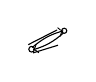
\begin{tikzpicture}[scale=.36]
\draw (0,0) circle (.10) (1.15,.65) circle (.09);
\draw[->] (.02,.06) to[bend left=12] (1.12,.65);
\draw[->] (1.12,.57) to[bend left=12] (.05,-.02);
\draw (-.12,.16)--(.90,.68) (.05,-.13)--(.93,.14);
\end{tikzpicture}}

Je résume le résultat obtenu

\uline{Proposition 10} Soit $Y$ une \inserted{petite} catégorie 1-connexe\inserted{, $y_0\in\mathrm{ob}\,Y$.} Alors $\underline{\mathrm{Ch}}(Y;y_0,-)$ est $W_\infty$-asphérique, mais n'est \inserted{pas} totalement $W_\infty$-asphérique si $Y$ elle-même n'est $\infty$-connexe \unsure{i.e.|ou} $W_\infty$-asphérique.

% slanted
\margin{Mais un exemple plus succinct est \diagram{\begin{tikzcd}[ampersand replacement=\&,column sep=small,row sep=small]
\&\&b\\
\unsure{\Psi|\Phi}={} \& a\arrow[ur]\arrow[dr]\&\\
\&\&c
\end{tikzcd}}, qui est $W_\infty$-asphérique, mais \uline{pas} totalement !}

On peut se demander si $Y$ $W_\infty$-asphérique implique que $\underline{\mathrm{Ch}}(Y;y_0,-)$ est tot. $W_\infty$-asphérique. J'en doute fort !
% archive sheet number: 154
\scanpage{155}
\mspage{104}

Revenons maintenant à la situation du début de la section, \deleted{\unsure{pour}} diagramme \unsure{$(x)$|$(\alpha)$} p. \unsure{87|82}

\diagram{\begin{tikzcd}[ampersand replacement=\&,column sep=small]
(x) \& U \arrow[r,hook,"i"] \arrow[d,"p"'] \& X \arrow[d,"q"'] \& T=\{t\} \arrow[l,dashed,"j"'] \arrow[d,dashed,"\mathrm{iso}"]\\
\& U' \arrow[r,hook,"i'"] \& X' \& T'=\{t'\}\arrow[l,dashed,"j'"']
\end{tikzcd}}

Nous pouvons donner maintenant un exemple où $i$ est dans $\unsure{W|\mathcal W}$ (et $=$ $W$-asphérique) sans que $i'$ le soit :

\[
i\in W,\ \deleted{\text{et}}\ i'\notin W.\tag*{\unsure{$(xx)$|$(x)'$|$(\alpha')$}}
\]

On peut $=$ supposer que $t$ soit objet final de $X$ (ce qui signifie que l'objet $H$ de $U^\wedge$ est \unsure{isomorphe} à $e_U$, l'objet final), et $t'$ objet final de $X'$ (i.e. $p_!(e_U)=e_{U'}$, i.e. les $ {}_{u'\backslash}U$ sont 0-asphériques). \deleted{Il suffit} Dans ce cas, comme $X,X'$ sont $W$-asphériques, les relations \unsure{$(xx)''$|$(xx)$|$(\alpha')$} équivalent à

\[
U\text{ est }W\text{-asphérique, et }U'\text{ non,}\tag*{\unsure{$(xxx)$|$(x'')$|$(\alpha'')$}}
\]

ce qui est justement la situation que nous venons de construire (p. 101--103).

On aimerait aussi trouver un exemple où dans $(x)$ on ait $p\in W$, $q\notin W$.
% archive sheet number: 155
\scanpage{156}
\mspage{105}

Je prendrai encore $(X,U,\{t\})$ tels que $t$ soit objet final de $X$, mais si on veut $q\notin\unsure{W|\mathcal W}$, on ne peut supposer $t'$ élément final de $X'$. Au lieu de cela, je vais supposer

a) $U,U'$ (et aussi $X$, ayant objet final $t$) $W$-asphériques donc \deleted{\unsure{$p$}} $i\in W$ (et $=$ $i$ $W$-asph.), $p\in W$, mais

b) $X'$ non $W$-asphérique, donc $i',q\notin W$.

Pour ceci, notons que,

\[
U'_{/t'}\simeq U'_{/p_!(e_U)}\overset{\mathrm{def}}{=}\underline{\unsure{\pi|\Pi}}_0(U/U'),
\]

le cor. de la prop. 7 (cf p. 85), non encore démontré, nous dit que $i'\in W$, \deleted{i.e.} (i.e. ici, $X'$\unsure{,} $W$-asph) ssi $i'$ est $W$-asph. i.e. $U'_{/t'}$ est $W$-asph. Nous allons l'admettre ici,

Tout revient donc à trouver une flèche

\[
p:U^{\unsure{4|*|+}}\longrightarrow U'
\]

dans $\mathrm{Cat}$ avec les propriétés suivantes

a) $U^4$ et $U'$ sont $W$-asphériques,

b) $\underline{\pi}_0(U^4/U')$ n'est pas $W$-asphérique.

Nous allons reprendre l'exemple précédent

\[
f:X\longrightarrow Y
\]

(p. 101 à 103), en \unsure{prenant|posant}

\[
U^4=X,\quad\underline{\pi}_0(U^4/U')=Y,
\]
% archive sheet number: 156
\scanpage{157}
\mspage{106}

donc \unsure{tout} revient, à partir de \inserted{l'exemple donné} $X\mathrel{\overset{f}{\unsure{-|\to}}}Y$, à construire une flèche

\[
\unsure{\pi|\Pi}:\deleted{\unsure{X}}Y\longrightarrow U'\tag*{\unsure{$(x)$|$(\alpha)$}}
\]

dans $\mathrm{Cat}$ qui satisfasse les conditions

a) $\pi$ est un iso. local \qquad b) $U'$ est \inserted{$\unsure{W|\mathcal W}$-}asphérique.

On prendra alors $p=\pi f$

Mais par la façon dont $X$ a été construit : partir d'un $Y$ 1-connexe et non $\infty$-connexe, \unsure{par} \deleted{\unsure{et}} ailleurs quelconque, on est ramené finalement à trouver $(x)$ satisfaisant a), b) et de plus

c) $Y$ est 1-connexe, mais non $\infty$-connexe

(NB on suppose maintenant $W=W_\infty$). Il revient au $=$ de trouver

% vertical rule at left
\noindent\makebox[0pt][r]{\rule[-1.8\baselineskip]{0.45pt}{2.6\baselineskip}\hspace{.65em}}%
$U'$ objet \uline{asph.} de $\mathrm{Cat}$, $F\in\mathrm{Ob}\,{U'}^\wedge$ tels que $U'_{/F}$ soit 1-connexe et non $\infty$-connexe.

On songe par exemple à prendre simplement une sous-catégorie ouverte $U'_0$ de $U'$, qui soit 1-connexe et non $\infty$-connexe. Partons d'une telle catégorie $U'_0$ -- par exemple une réalisation \inserted{homotopique} dans $\mathrm{Cat}$, de la sphère $S^2$. On l'immerge \inserted{comme ouvert} dans un $U'$ asphérique, en lui ajoutant un objet final. On a gagné !
% archive sheet number: 157
\scanpage{158}
\mspage{107}

Faisons un énoncé en forme

\uline{Proposition 11} On peut trouver une situation \unsure{$(x)$|$(\alpha)$} (p. 124) avec

a) $t$ objet final de $X$

b) $U,U'$ (et $X$) $\unsure{W|\mathcal W}_\infty$-asphériques, donc $i,p\in W_\infty$ \inserted{(et même $i$ $W_{\unsure{\infty|0}}$-asphérique)}

c) $X'$ non $W_\infty$-asphérique, donc $i',q\notin W_\infty$.

Il suffit pour cela de partir d'un objet 1-connexe \deleted{et non $\infty$-connexe} $Y$ de $\mathrm{Cat}$, de lui adjoindre un objet final \inserted{$u'_0$}, ce qui donne $U'$, de prendre $U=\underline{\mathrm{Ch}}(Y;y_0,-)$, $p:U\to U'$ le composé $U\xrightarrow{\mathrm{but}}Y\mathrel{\mathop{\hookrightarrow}\limits^{\mathrm{incl.}}_{\mathrm{can}}}U'$, et $X$ \unsure{se} déduit de $U$ en lui ajoutant un objet final $t$. On a alors $U'_{/t'}\simeq Y$, \deleted{(\unsure{donc} si $Y$ était $\infty$-connexe)} d'où

\[
 X'\ W_\infty\text{-asph}\quad (\text{i.e. }i'\in W_\infty)\Longleftrightarrow Y\quad W_\infty\text{-asphérique.}
\]

On a le contr'exemple cherché en prenant $Y$ \deleted{(1-connexe mais)} non $\infty$-connexe.

\uline{2.4.} \uline{Application aux immersions ouvertes dwyériennes}

Donnons avant $=$ l'énoncé \uline{positif} auquel nous en \unsure{arrivons|étions}.

\uline{Théorème 3} Soient $(X,U,T)$ un triple $\in\unsure{\mathscr T|\mathcal T}$ ($U$ ouvert de $X$ dans $\mathrm{Cat}$, $T=X-U$), \inserted{et pour \unsure{la} \deleted{\unsure{toute}} flèche} $p:U\longrightarrow U'$ \deleted{\unsure{une}} flèche de $\mathrm{Cat}$, \deleted{\unsure{soit}} le carré cocartésien dans $\mathrm{Cat}$

\diagram{\begin{tikzcd}[ampersand replacement=\&,column sep=small]
U \arrow[r,hook,"i"] \arrow[d,"p"'] \& X \arrow[d,"q"'] \& T \arrow[l,dashed,hook] \arrow[d,dashed,"\mathrm{iso}"]\\
U' \arrow[r,"i'"] \& X' \& T' \arrow[l,dashed,hook]
\end{tikzcd}}
% archive sheet number: 158
\scanpage{159}
\mspage{108}

Supposons que pour \deleted{tout} $t\in \unsure{\dot T|T}\inserted{{}=\bar U}$, le \deleted{\unsure{foncteur}} préfaisceau

\[
\deleted{i_0^{*}(t)\longrightarrow\unsure{\cdot|{}}}
\]

\[
i^{*}(t)=(u\longmapsto\operatorname{Hom}_{X}(u,t))\in U^{\wedge}
\]

soit $\unsure{W|\mathcal W}$-asph. \inserted{(déf. 1 p. 88*)} -- \unsure{p. ex.|i.e.} que la catégorie $U_{/t}$ soit tot. $W$-asph. (prop 8 page 93).

% slanted
\margin{\uline{NB} On dit \unsure{alors} sous ces conditions que $i_0:U\mathbin{-}\bar U$ est \uline{strictement} \deleted{\unsure{tot.}} \uline{$W$-asphérique} (cf déf. 2 page suivante)}

[ NB Le cas où les $U_{/t}$ ont un objet final, cf prop 9 a) i.e. celui où \unsure{l'immersion} $U\to\bar U$ admet un adjoint à droite, est celui envisagé \deleted{\unsure{dans}} chez Dwyer \deleted{\unsure{pour ce}} \deleted{\unsure{avec}} les \uline{imm. ouvertes}

\uline{de Dwyer}\inserted{*})

% slanted
\margin{Je ne connais pas d'autre cas où le th. soit susceptible de s'appliquer, -- les exemples de catégories tot. $W$-asphériques qui n'ont un objet final, \unsure{mais} sont qd même tot. $W$-asphériques, \unsure{$F$|$R$} d'une catégorie $U^{\wedge}$, \unsure{que} je sais sont les $U_{/F}$ où $U$ \unsure{n'importe|quelconque} et $F$ un objet \unsure{filtrant}, ou pour être précis tels que $F$ soit, \unsure{comme} les catégories \uline{filtrantes} sont tot. $W$-asph. si $W$ satisfait \unsure{à des axiomes}, cf démonstration plus loin, en \unsure{des circonstances}, -- p. 112.}

Alors pour tt $f:U\mathbin{-}U'$, l'immersion ouverte

\[
U'\mathbin{-}\bar U'
\]

\unsure{$W$-asphérique} est $=$, \inserted{tout} comme $i_0$, \deleted{\unsure{total}}strictement $W$-asphérique), et a fortiori elle est \unsure{totale|cohér}. \unsure{Par suite|D'ailleurs} (prop. 5) on a ceci

\[
\begin{aligned}
\text{\textcircled{a}}\quad i\in W &\iff i'\in W &&\text{moyennant }W(7\text{ bis})\\
\text{\textcircled{b}}\quad p\in W &\iff q\in W &&\text{moyennant }W(7).
\end{aligned}
\]

\uline{Corollaire 1} \inserted{Supposons $W(7)$.} Si $i:\deleted{\unsure{A}}U\longrightarrow X$ est une imm. ouverte telle que $i_0:U\mathbin{-}\bar U$ soit tot. $W$-asph., \deleted{\unsure{alors}} alors \inserted{$i:U\mathbin{-}X$ est} une $W$-\uline{cofibration} \inserted{(``ultra forte'')}, par quoi j'entends ceci :

pour ttes flèches $U'\xrightarrow{f}U''$ dans $U\backslash\mathrm{Cat}$,
% archive sheet number: 159
\scanpage{160}
\mspage{109}

telle que $p\in\unsure{W|\mathcal W}$, la flèche $g:X'\mathbin{-}X''$ qui s'en \unsure{déduit} par cochangement de base à partir de l'objet $X$ de $U\backslash\mathrm{Cat}$, est aussi dans $W$.

\uline{Dém. du corollaire} : on applique le th. 3 à l'immersion ouverte $U'\overset{i'}{\hookrightarrow}X'$ \unsure{déduite} de $U\overset{i}{\hookrightarrow}X$ par le cochangement de base $U\xrightarrow{p}U'$, en notant de plus que l'hypothèse du th. 3 sur $i$ est \unsure{préservée} en passant de $i$ à $i'$.

Il faut \unsure{quand} même introduire une terminologie adéquate :

\uline{Définition 2} : a) Une flèche $f:X\mathbin{-}Y$ est dite \uline{strict\deleted{\unsure{em}}ement $W$-asph.} si pour tout $y\in\operatorname{Ob}Y$, $f^{*}(y)=(x\longmapsto\operatorname{Hom}_{Y}(f(x),y))$ est un objet \unsure{tot.} $W$-asph. de $X^{\wedge}$ (cf déf. 1 page 88). Elle est dite \deleted{strictement} \uline{totalement} $W$-\uline{asphérique} si, pour tout $y\in\operatorname{Ob}Y$, $\mathrm{cat.}\ X_{/y}\ (\simeq X_{/f^{*}(y)})$ est \deleted{\unsure{t}}un objet \unsure{tot.} $W$-asphérique \unsure{de|ds}.

b) Une immersion ouverte $i:U\mathbin{-}X$ est dite \deleted{\unsure{(faiblement)}} \inserted{$W$-}dwyérienne, \inserted{(resp. \deleted{totalement} dwyérienne)} \inserted{si} l'immersion \unsure{induite} $i_0:U\mathbin{-}\bar U$ est \deleted{\unsure{strict}}strictement \inserted{(resp. totalement)} \uline{$W$-asphérique}. Une immersion fermée est \deleted{\unsure{dite ou non}} \inserted{$j:J\mathbin{-}X$} est dite \inserted{$W$-}dwyérienne (resp. tot. $W$-dwyérienne) ssi $j^{\mathrm o}:\unsure{I|J}^{\mathrm o}\mathbin{-}X^{\mathrm o}$ est une imm. ouverte $W$-dwyérienne (resp. tot. $W$-dwyérienne).

c) Une \deleted{\unsure{immersion ouverte ou fermée est}} \inserted{flèche $i:U\mathbin{-}X$ \unsure{ds|de} $\mathrm{Cat}$ (pas néc. une imm.)}
% archive sheet number: 160
\scanpage{161}
\mspage{110}

est appelée une $\unsure{W|\mathcal W}$-cofibration, si pour tte flèche $f:\deleted{\unsure{A}}U'\longrightarrow U''$ dans $U\backslash\mathrm{Cat}$, la flèche $g:X'\mathbin{-}X''$ qui s'en déduit par le coch. de base \deleted{\unsure{par|sur}} $X$ (objet de $U\backslash\mathrm{Cat}$) est dans $W$ quand $f$ l'est.

\uline{NB} Cette notion \inserted{de $W$-cofibration} est stable par composition et par cochangement de base, et les iso. de $\mathrm{Cat}$ sont des $W$-cofibrations. Si $f$ est une $W$-cofibration, $f^{\mathrm o}$ l'est et inversement.

[ Le corollaire s'énonce en disant qu'une imm. ouverte ou fermée qui est \inserted{$W$-}dwyérienne est une $W$-cofibration. ]

d) Une flèche $i:U\mathbin{-}X$ dans $\mathrm{Cat}$ est appelée une \uline{$W$-cofibration triviale}, ou une $W$-\uline{équivalence couniverselle}, si pour tout $U'$ dans $U\backslash\mathrm{Cat}$, i.e. \deleted{\unsure{tout}} flèche $\unsure{p|f}:U\mathbin{-}U'$ dans $\mathrm{Cat}$, la flèche déduite de $i$

\[
i':U'\mathbin{-}X'=U'\amalg_{U}X'
\]

est dans $W$. (NB Il est immédiat que cela \unsure{entraîne|entraîne,} bien que $i$ est une $W$-cofibration.) [ Cette notion de $W$-cofibration triviale est elle aussi stable par composition et par cochangement de base, et les iso de $\mathrm{Cat}$ en sont. ]
% archive sheet number: 161
